\documentclass[../report.tex]{subfiles}

\begin{document}
\graphicspath{{img/}{../img/}}


\section{Gantt planl�gning}
Gantt er en udbyggelse af den klassiske tidsplan. Den er lavet for at give et bedre overblik over de forskellige planlagte opgaver i forhold til hinanden. Hvor en klassisk tidsplan i form af en tabel er fokuseret p� tidsperioderne, er et Gantt diagram fokuseret p� arbejdsopgaverne.\\

P� side \pageref{fig:Gantt} ses Gantt diagrammet for target projektet. Diagrammet er lavet p� baggrund af tidligere erfaringer og presset fra den faste deadline.\\ \\


\begin{figure}[H]
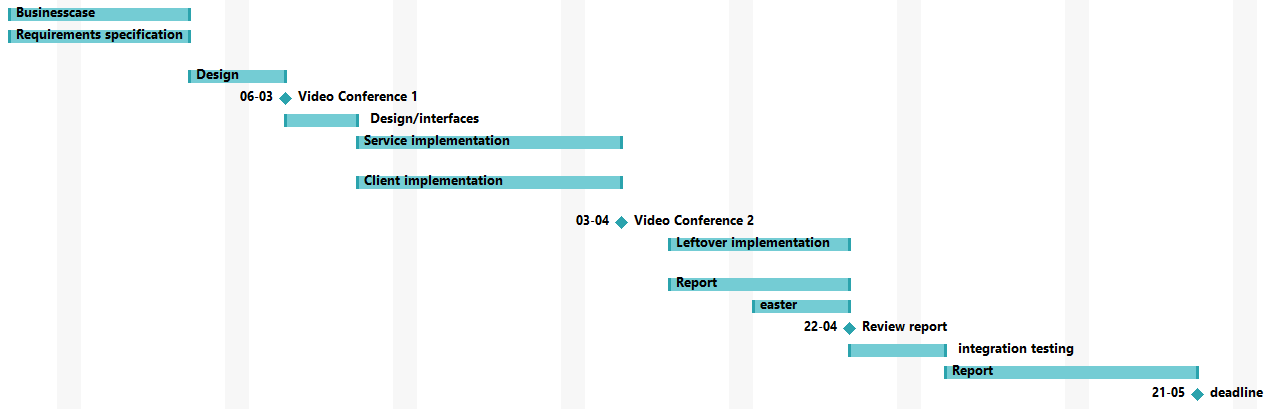
\includegraphics[scale=0.45]{TargetProjectGantt.png}
\label{fig:Gantt}
\end{figure}

I et eksamensprojekt er deadlinen fast, og m�let for planl�gningen er alts� ikke at se hvorn�r vi kan v�re f�rdige, men hvorn�r delarbejdsopgaver cirka skal v�re f�rdige for at vi kan n� deadlinen. Den n�dvendige arbejdsindsats kan alts� varierer alt efter hvad man l�bende kan se er n�dvendigt for at overholde arbejdsopgavernes perioder som specificeret i Gantt diagrammet.







\end{document}